\section{Versuchsaufbau}
\label{sec:Versuchsaufbau}
\nocite{Halbleiter}
\begin{figure}[H]
  \centering
  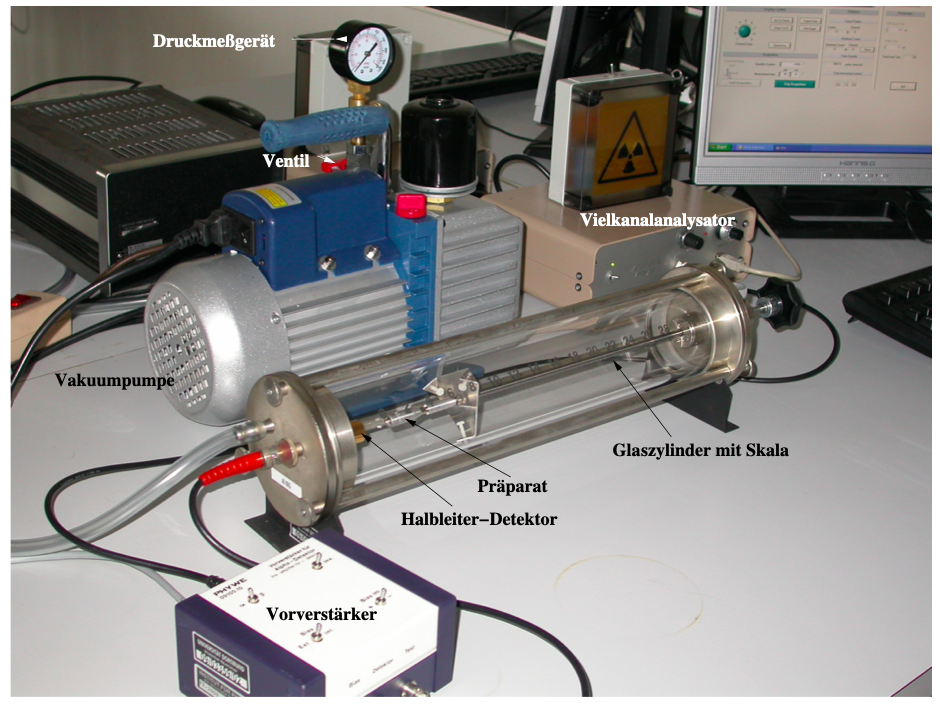
\includegraphics[width=0.7\textwidth]{content/Bilder/Messapparatur.png}
  \caption{Versuchsaufbau zur Bestimmung der Reichweite von $\alpha$-Strahlung Q\cite{anleitungV701}.}
  \label{fig:Messapparatur}
\end{figure}
Der Versuch wird mithilfe der Apparatur in Abbildung \ref{fig:Messapparatur} durchgeführt. In dem Glaszylinder 
befindet sich ein $\alpha$-Präparat sowie ein Detektor, deren Distanz $x_0$ einstellbar ist. In diesem Fall wird als 
Strahlungsquelle ein \ce{Am}-Präparat verwendet. Bei diesem Versuch ist der Deketor ein Halbleiter-Sperrschichtzähler, welcher an eine 
Gleichspannung in Sperrrichtung angelegt ist und ähnlich wie eine Diode funktioniert. Ein Halbleiter-Sperrschichtzähler besteht aus
n- und p-Leitern zwischen denen sich eine ladungsträgerfreie Zone (Verarmungszone) bildet. Diese Zone wird durch eine Spannung in Sperrichtung vergrößert. 
Ein Strompuls ensteht, indem ein einfallendes Ion in der Verarmungszone mehrere Elektronen-Loch Paare erzeugt. Der enstehende Puls wird durch einem
Vorverstärker verstärkt und mithilfe eines Vielkanalanalysators die zugehörige Pulshöhe ermittelt. Außerdem ist der obige Versuchsaufbau
mit einem Computer verbunden. Darauf wird mithilfe des Programms \textit{Multichannel Analyzer} und mit eingestelltem \textit{Multichannel Analysator} (\textit{MCA})
kann die Gesamtzählrate gemessen und eine Pulshöhenanalyse durchgeführt werden. Bevor die Messung beginnt, werden die Diskreminatorschwellen
am Vielkanalanalysator eingestellt. Dafür wird der Abstand zwischen der Quelle und dem Detektor auf ca. $4$ bis $5\,\unit{\centi\metre}$ eingestellt. 
Anschließend wird die Schwelle angepasst, sodass bei Atmosphärendruck unter \textit{pulses detected} Pulse zu erkennen sind. 

\section{Durchführung}
\label{sec:Durchführung}
Zunächst wird der Glaszylinder Evakuiert, indem die Belüftungsventile geschlossen werden und die Drehschieberpumpe aktiviert 
wird. Sobald der Druck bei $p \approx 0\,\unit{\milli\bar}$ liegt, wird das rote Ventil zwischen der Pumpe und dem Glaszylinder 
geschlossen und die Pumpe ausgestellt. Wenn der Druck in der Apparatur konstant bleibt, kann die Messung beginnen. Um die Reichweite 
von $\alpha$-Strahlung zu bestimmen, wird die Energieverteilung und die Zählrate der $\alpha$-Strahlung in Abhängigkeit vom Druck $p$ 
in Abständen von ca. $50\,\unit{\milli\bar}$ gemessen. Der Druck wird mithilfe des Belüftungsventils eingestellt und die Messzeit beträgt $2\,\unit{\minute}$. 
Für jede Messung wird die Position des Energiemaximums und die Gesamtzählrate notiert. 
Diese Messungen werden für zwei verschiedene Abstände zwischen dem Detektor und der $\alpha$-Strahlung durchgeführt. Anschließend wird 
eine Messreihe zur Überprüfung der Statistik des radioaktiven Zerfalls aufgenommen. Dabei wird der Glaszylinder erneut evakuiert und es 
werden 100 mal die Zerfälle pro Zeiteinheit bei einem Druck von $p = 0\,\unit{\milli\bar}$ gemessen. Die Messzeit beträgt hier $10\,\unit{\second}$.
